\documentclass[12pt]{article}
\usepackage[utf8]{inputenc}
\usepackage[left=2cm,right=2cm,top=2cm,bottom=2cm]{geometry}
\usepackage{graphicx, color}
\usepackage{subcaption}
%\usepackage[small]{caption}
\usepackage[spanish]{babel}
\usepackage{url}
\setlength{\parskip}{\baselineskip}
\graphicspath{ {images/} }


\usepackage{hyperref}
\hypersetup{
	colorlinks=true,
	linkcolor=blue,     
	urlcolor=blue,
	citecolor=blue,
}


\begin{document}


	\thispagestyle{empty}

	\begin{center}
		{\Large Frecuencias}\\ % e histogramas}\\
		Gabriela S\'anchez Y.\\
		5064
	\end{center}

	En el presente trabajo se realiza un análisis del libro \textit{``Anne of Green Gables''} obtenido del sitio de \href{http://www.gutenberg.org/}{Project Gutenberg}. 

	\section{Introducción}
	
	El análisis del libro de texto se realiza con la ayuda del lenguaje de programación \textsc{R} versión 4.0.2 \cite{r}, haciendo uso de tres librerías: \texttt{gutenbergr} que permite acceder al texto plano del libro y, \texttt{tidytext} y \texttt{dplyr} que permiten la descomposición del texto.

	Dicho análisis se basa en el estudio de las frecuencias de las palabras y letras del texto. El primer paso para poder proceder con el estudio es obtener el texto plano del libro, lo cual es posible mediante la función \texttt{gutenberg\_download}.  

	\section{Letras}
	
	La descomposición del texto en caracteres se realiza con la función \texttt{unnest\_tokens}. Ya que es de interés únicamente la frecuencia de las letras, se eliminan todos los caracteres que no lo son. En este caso, el único caracter que no es una letra es ``$\mid$". 
	
	Para mejorar la visualización, las frecuencias se ordenan en forma decreciente. De esta manera es posible observar que las primeras tres letras más usadas en el texto son \textit{e, t} y \textit{a}, mientras que las menos usadas son \textit{x, q} y \textit{z}, tal y como se muestra en la figura \ref{letras}.
	
	
	\begin{figure}
		\centering
		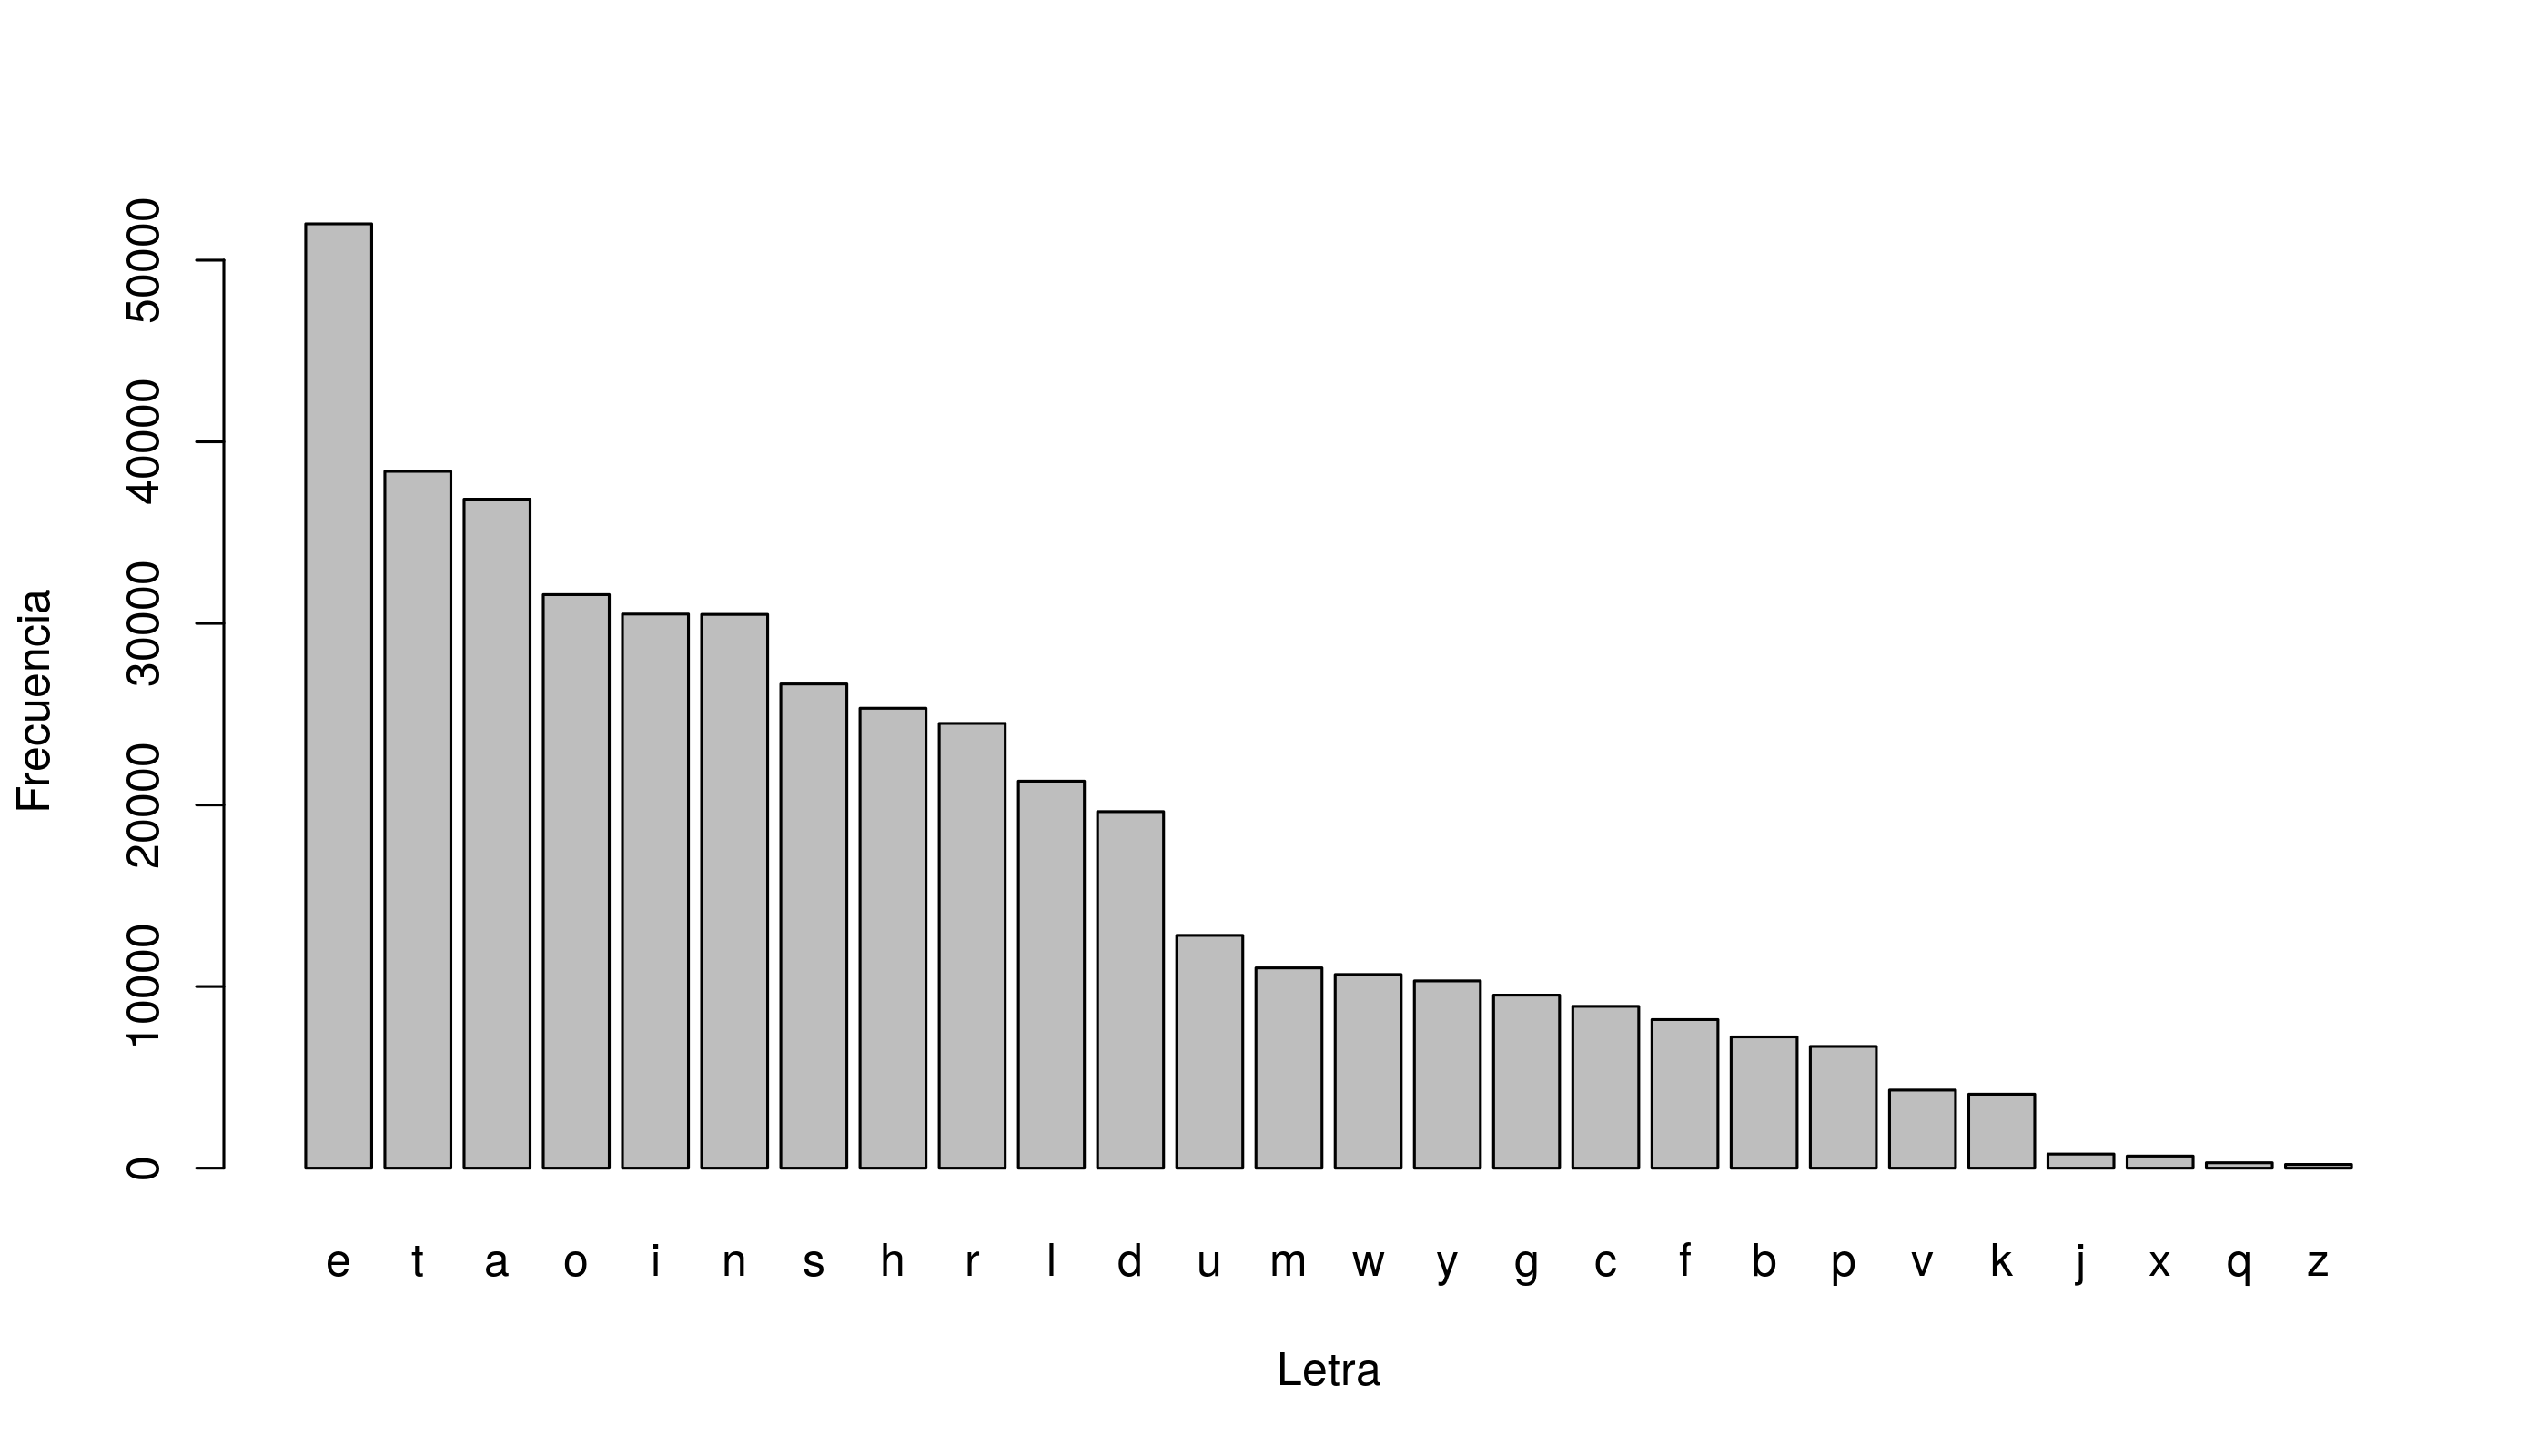
\includegraphics[scale=0.7]{letras_decreciente.png}
		\caption{Gráfico de barras de la frecuencia de las letras del abecedario en el texto analizado.}
		\label{letras}
	\end{figure}

	\section{Palabras}
	
	La descomposición en letras no dice mucho acerca del texto por lo que se procede a realizar una descomposición en palabras. Para esto, nuevamente se usa la función \texttt{unnest\_tokens}.
	
	Como segundo paso en este análisis, se realiza un filtrado: son eliminadas aquellas palabras que en inglés se conocen como \textit{stop words} (palabras vacías), ya que no serán útiles para el estudio \cite{textMining}. Son palabras muy comunes en el idioma que pueden eliminarse sin sacrificar el significado de una oración. En inglés algunos ejemplos de palabras vacías son \textit{at, the, is, of, to}.
	
	Una vez hecho este filtro, se aplica otro que toma en cuenta únicamente las palabras con una frecuencia mayor a uno. En el cuadro \ref{frecuencia_palabras} se pueden observar las primeras 10 palabras más frecuentes. Estos resultados permiten inferir que \textit{Anne, Marilla, Diana} y \textit{Matthew} son personajes principales en la novela, siendo \textit{Anne} el principal ya que la frecuencia está muy por encima de los otros.
	
	\begin{table}
		\centering
		\caption{Palabras más comunes y su frecuencia.}
		\label{frecuencia_palabras}
		\begin{tabular}{l|l}
			\hline
			Palabra & Frecuencia \\
			\hline
			anne & 1107\\
			marilla & 797\\
			diana & 386\\
			matthew & 339\\
			time & 178\\
			girl & 170\\
			school & 152\\
			miss & 148\\
			home & 144\\
			white & 142\\
			\hline
		\end{tabular}
	\end{table}

	Continuando con las palabras más frecuentes, en la figura \ref{palabras_dec} se muestra un gráfico de barras que muestra la frecuencia de las 20 palabras siguientes en frecuencia a las del cuadro \ref{frecuencia_palabras}. Pueden observarse otros nombres como \textit{Gilbert y Jane} y, lo que parecen ser apellidos \textit{Lynde} y \textit{Barry}, por lo que podríamos decir que son personajes secundarios en la novela. 
	
	\begin{figure}
		\centering
		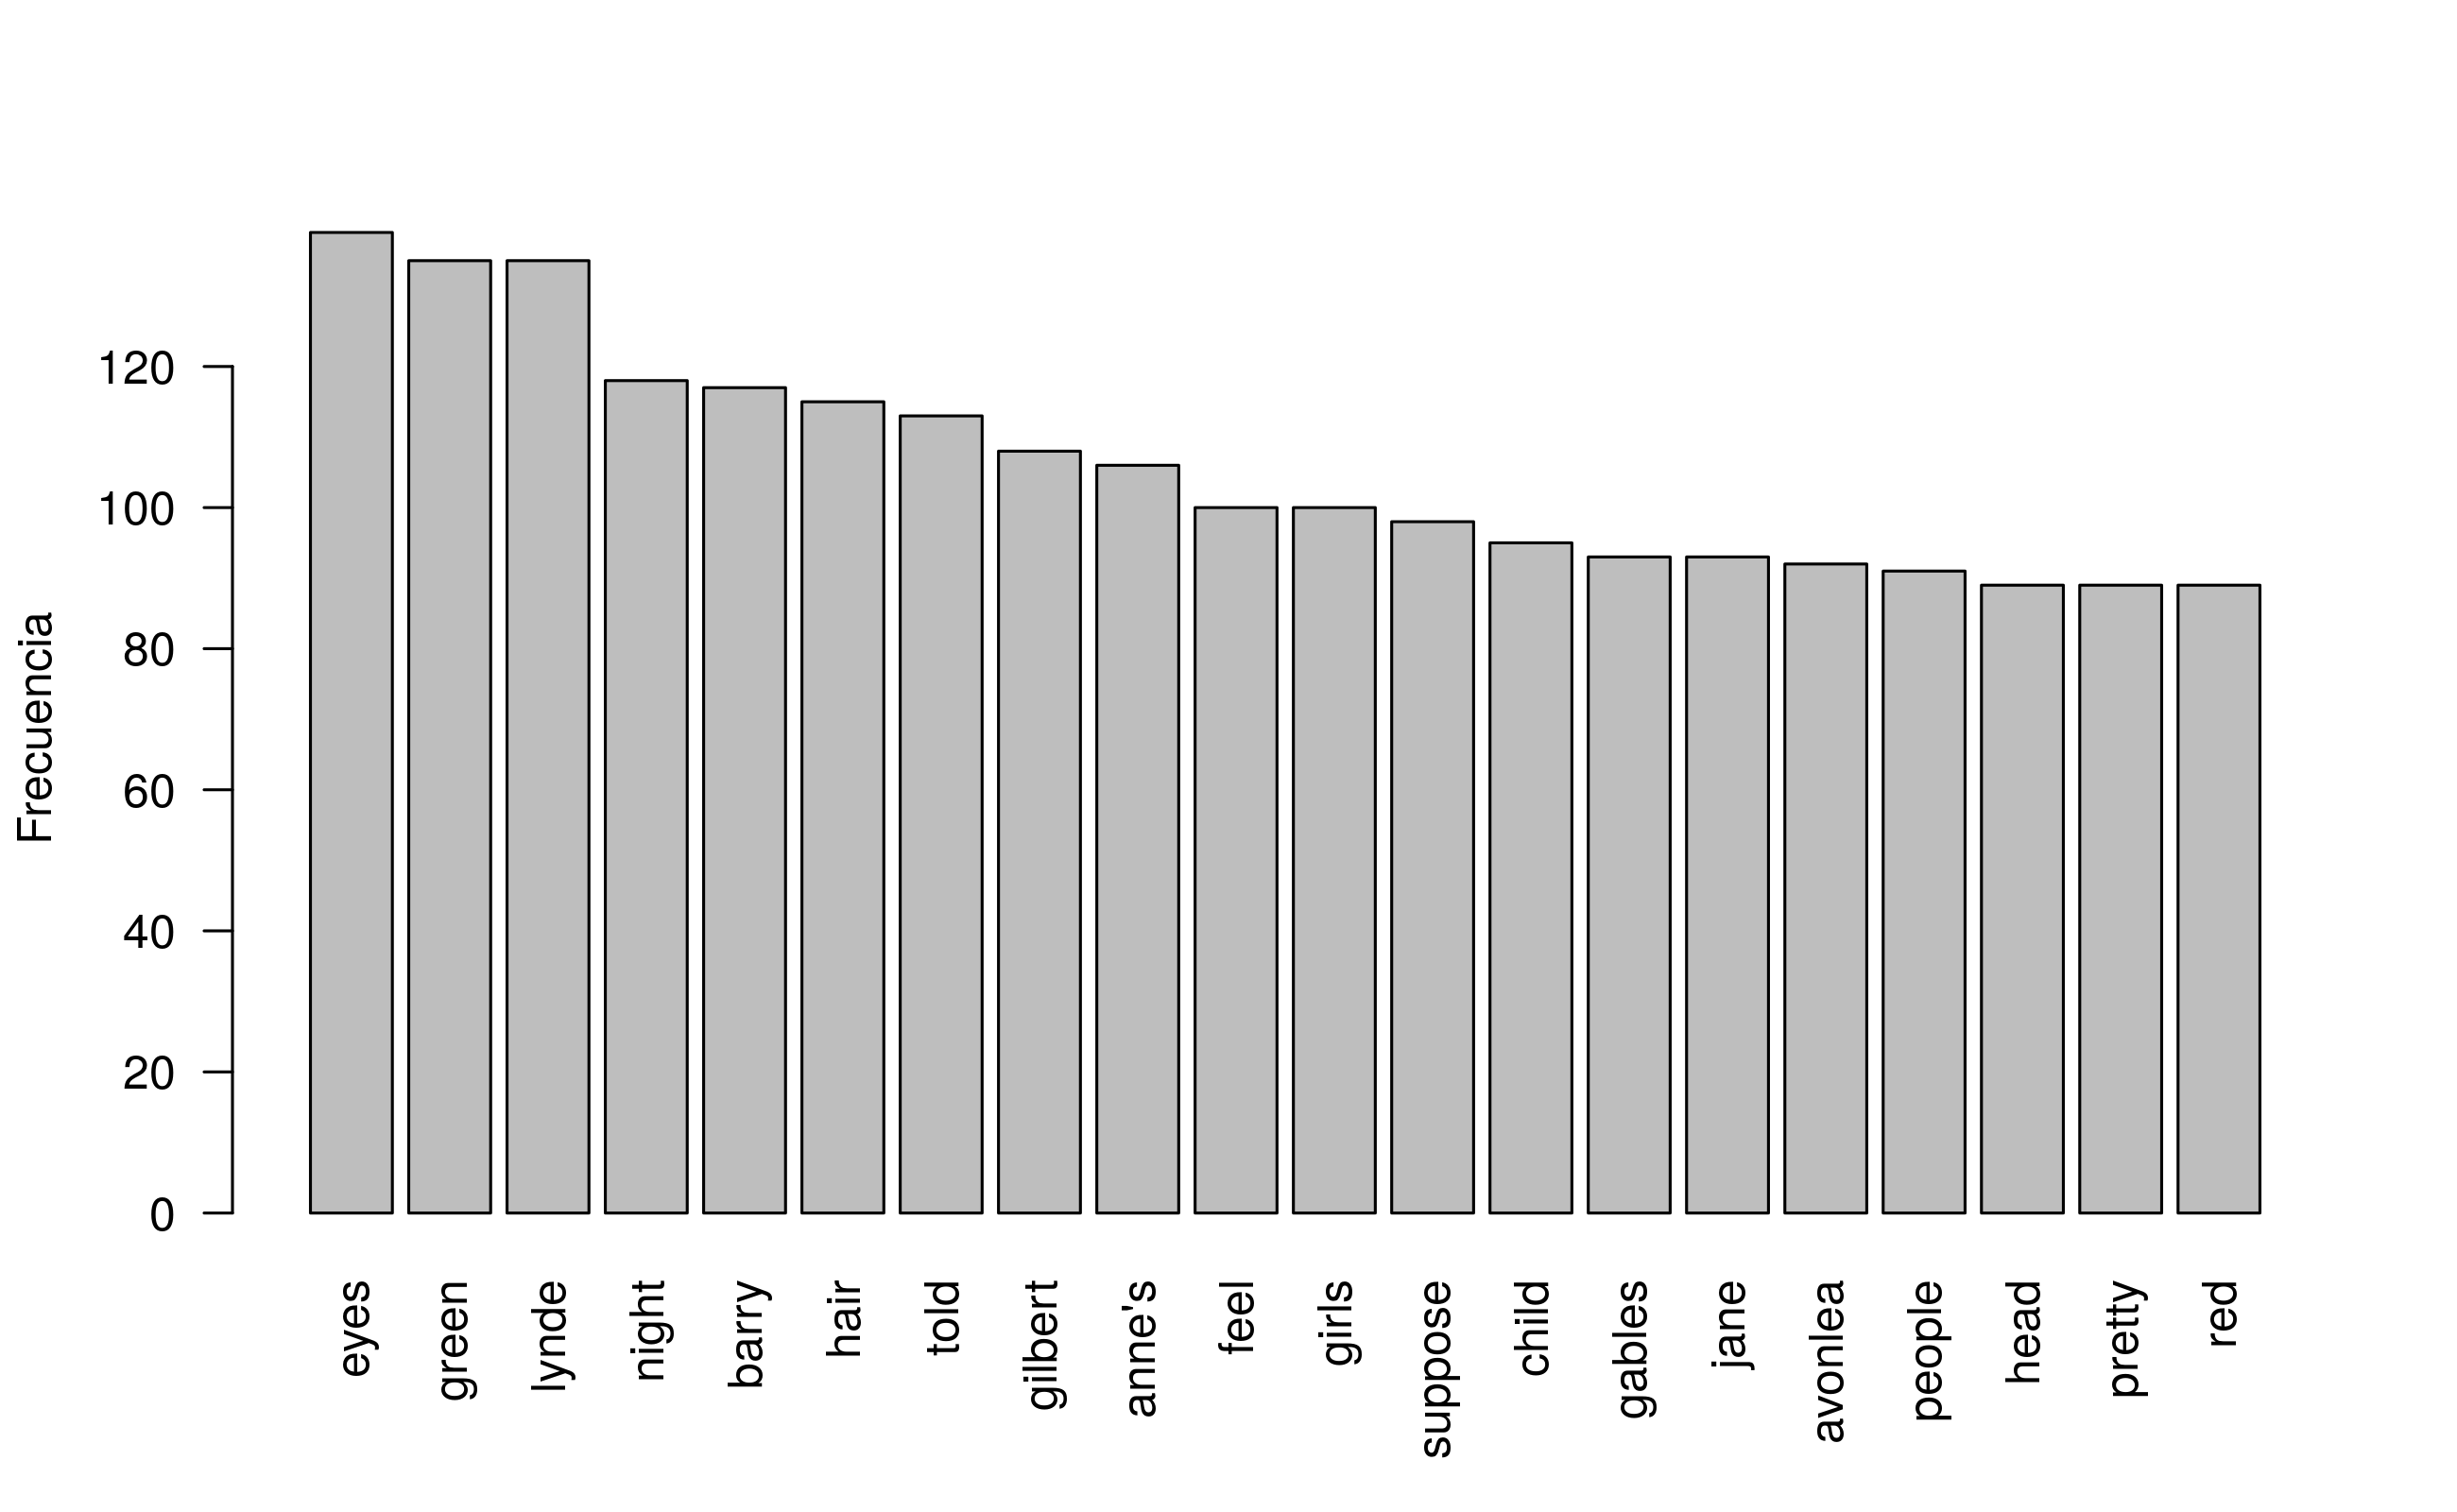
\includegraphics[scale=0.7]{palabras_decreciente_log3.png}
		\caption{Gráfico de barras de las palabras más frecuentes en el texto, una vez realizados dos filtros.}
		\label{palabras_dec}
	\end{figure}
	
	Una persona que ya ha leído el libro sabe que \textit{Barry} es el apellido de \textit{Diana}. Esto advierte que un análisis de palabras ``sueltas'' no permite inferir mucho acerca del contenido del texto, una mejor opción es considerar la frecuencia en que aparecen dos o más palabras juntas.
	
	Antes de proceder a analizar conjuntos de palabras, se examinan las palabras positivas y negativas más comunes de acuerdo al léxico \texttt{bing}, que es posible obtener a través de la función \texttt{get\_sentiments}. La figura \ref{palabras_pos-neg} muestra las 10 palabras más comunes positivas (figura \ref{palabras_positivas}) y negativas (figura \ref{palabras_negativas}). 
	
	En el gráfico de barras mostrado en la figura \ref{palabras_negativas} se puede apreciar que la palabra negativa con más frecuencia en el libro es \textit{miss}. Sin embargo, aquí se señala un problema. Se sabe que tanto en español como en inglés existen palabras homónimas, es decir, palabras cuya pronunciación o escritura es igual o similar pero que tienen diferente significado. En este caso, personas que ya han leído el libro, pueden advertir que el personaje principal se refiere a su profesora como \textit{Miss Stacy}, otro personaje relevante en la novela. por lo que no se garantiza que \textit{miss} en su connotación ``negativa'' realmente tenga una frecuencia más alta que las otras palabras mostradas en el gráfico.
	
	\begin{figure}
		\begin{subfigure}{.5\textwidth}
			\centering
			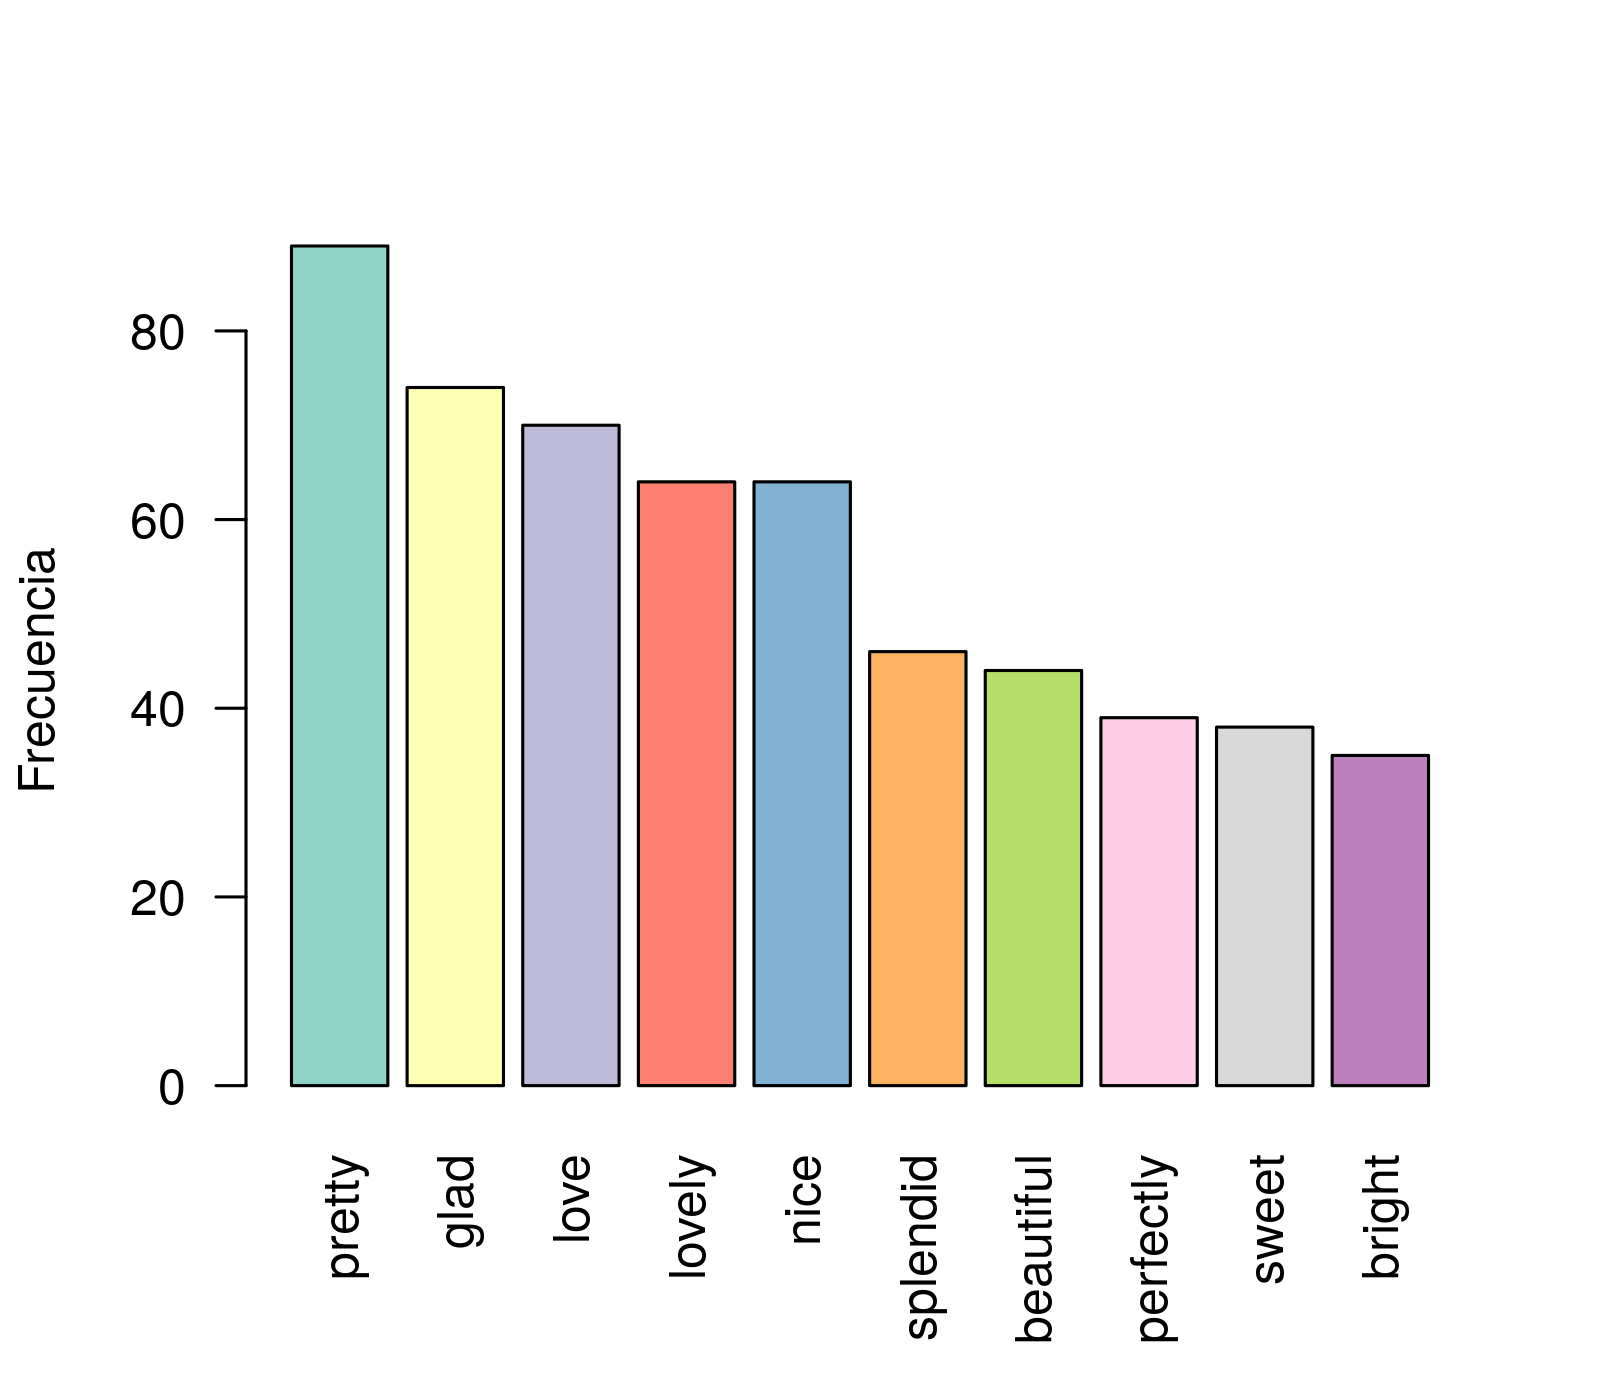
\includegraphics[width = 0.9\linewidth]{palabras_positivas.png}
			\caption{Palabras positivas}
			\label{palabras_positivas}
		\end{subfigure}
		\begin{subfigure}{0.5\textwidth}
			\centering
			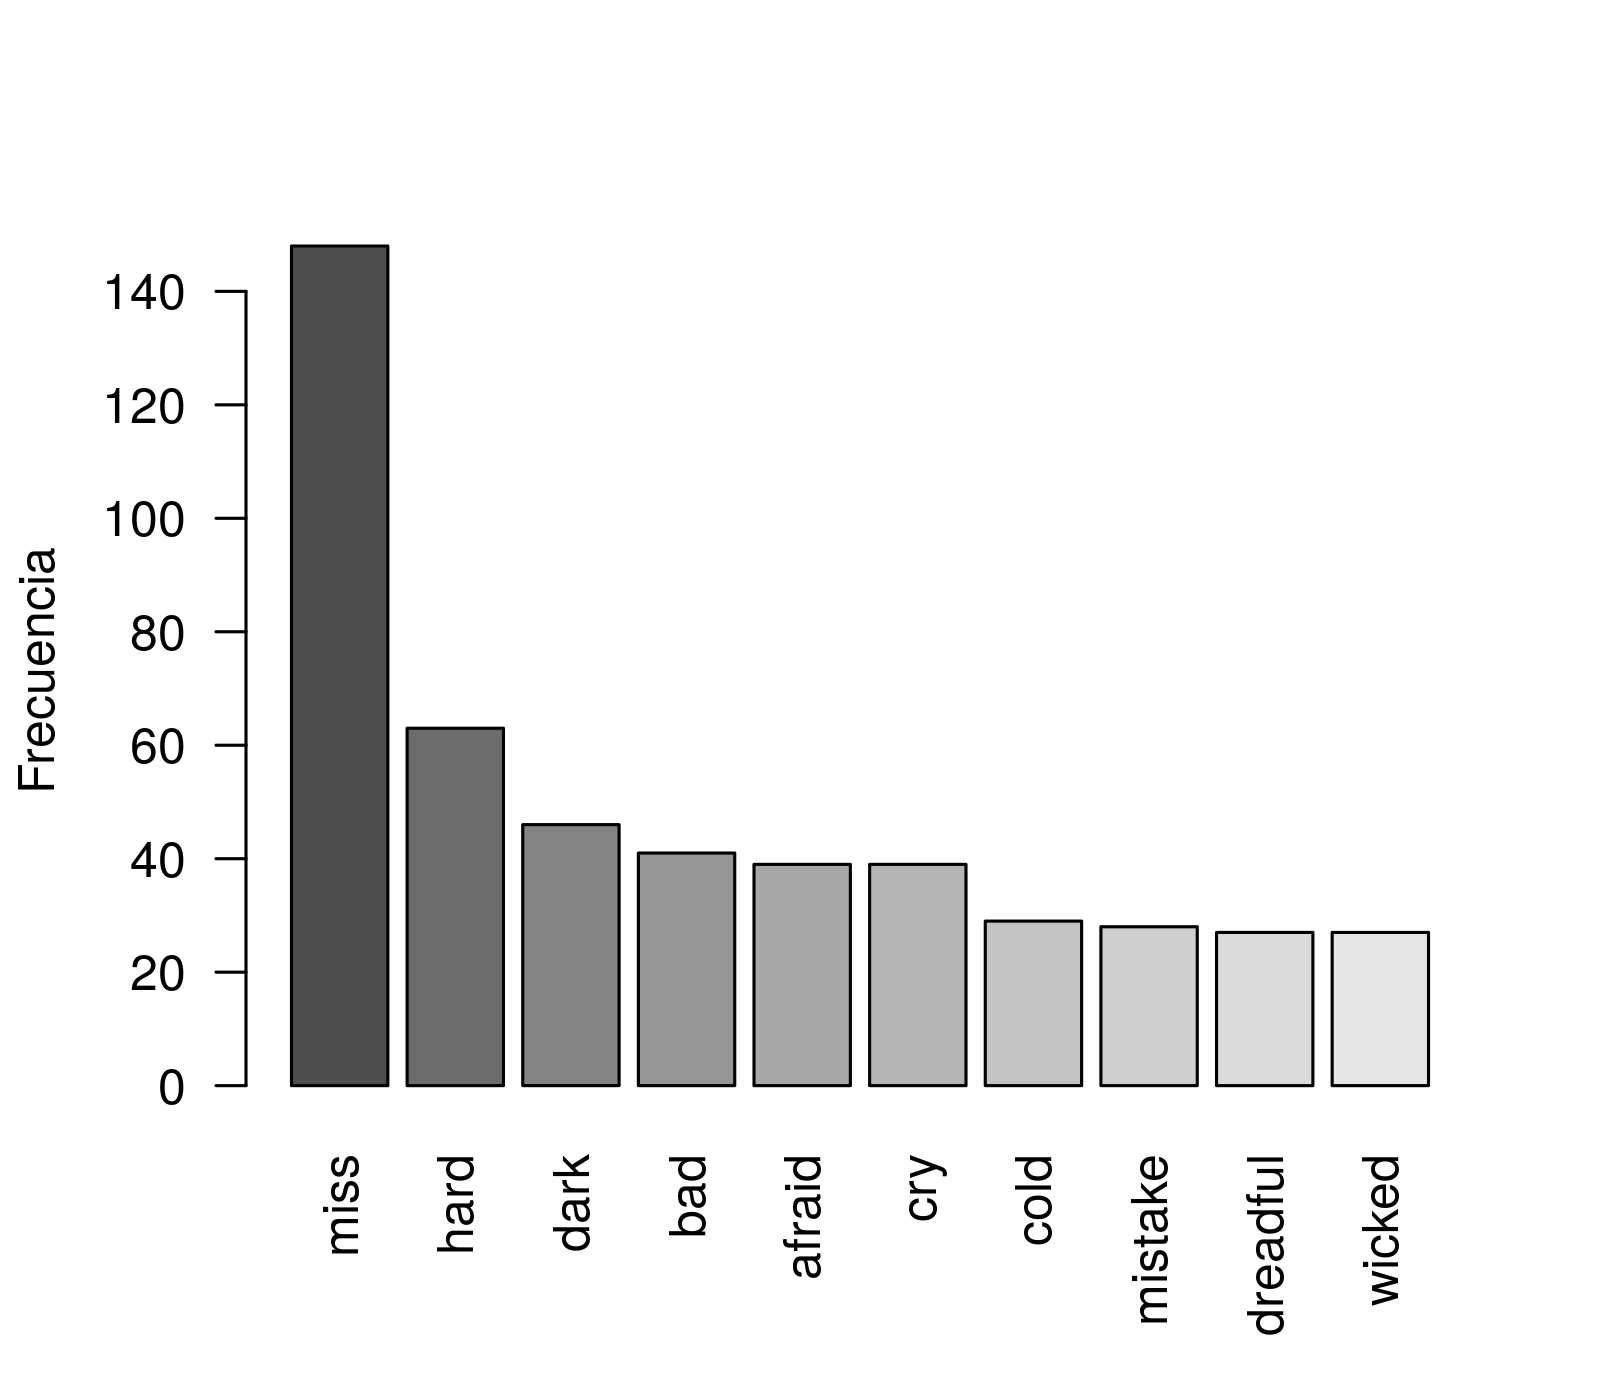
\includegraphics[width = 0.9\linewidth]{palabras_negativas.png}
			\caption{Palabras negativas}
			\label{palabras_negativas}
		\end{subfigure}
	
		\caption{Gráfico de barras de las palabras positivas y negativas más frecuentes.}
		\label{palabras_pos-neg}
	\end{figure}
	
	Por último, se analiza la frecuencia en que aparecen las secuencias de dos palabras, también llamado bigrama. El análisis de los brigramas se realiza con los datos que previamente filtraron las palabras vacías, ya que si se omite ese paso, los resultados obtenidos muestran serán los que se muestran en el cuadro \ref{frecuencia_bigramas} y dicha información no aporta sobre el contenido del libro.
	
	\begin{table}
		\centering
		\caption{Bigramas más frecuentes en el texto sin filtro.}
		\label{frecuencia_bigramas}
		\begin{tabular}{l|l}
			\hline
			Bigrama & Frecuencia \\
			\hline
		  	in the  &   413 \\
			to be    &  325 \\
		 	of the   &  308 \\
		 	it was   &  273 \\
		 	to the   &  240 \\
		 	and i    &  198 \\
		 	on the   &  191 \\
		 	i don't  &  174 \\
		 	going to &  165 \\
		 	was a    &  164 \\
			\hline
		\end{tabular}
	\end{table}

	En la figura \ref{bigrama_barplot} se observan los bigramas más comunes en el texto filtrado. Resalta el nombre de \textit{Green Gables}, lugar donde se desarrolla la mayoría de la trama de la novela y nombres de personajes como \textit{Miss Stacy,  Gilbert Blythe, Anne Shirley, Rubby Gillis,} entre otros.
	
	\begin{figure}
		\centering
		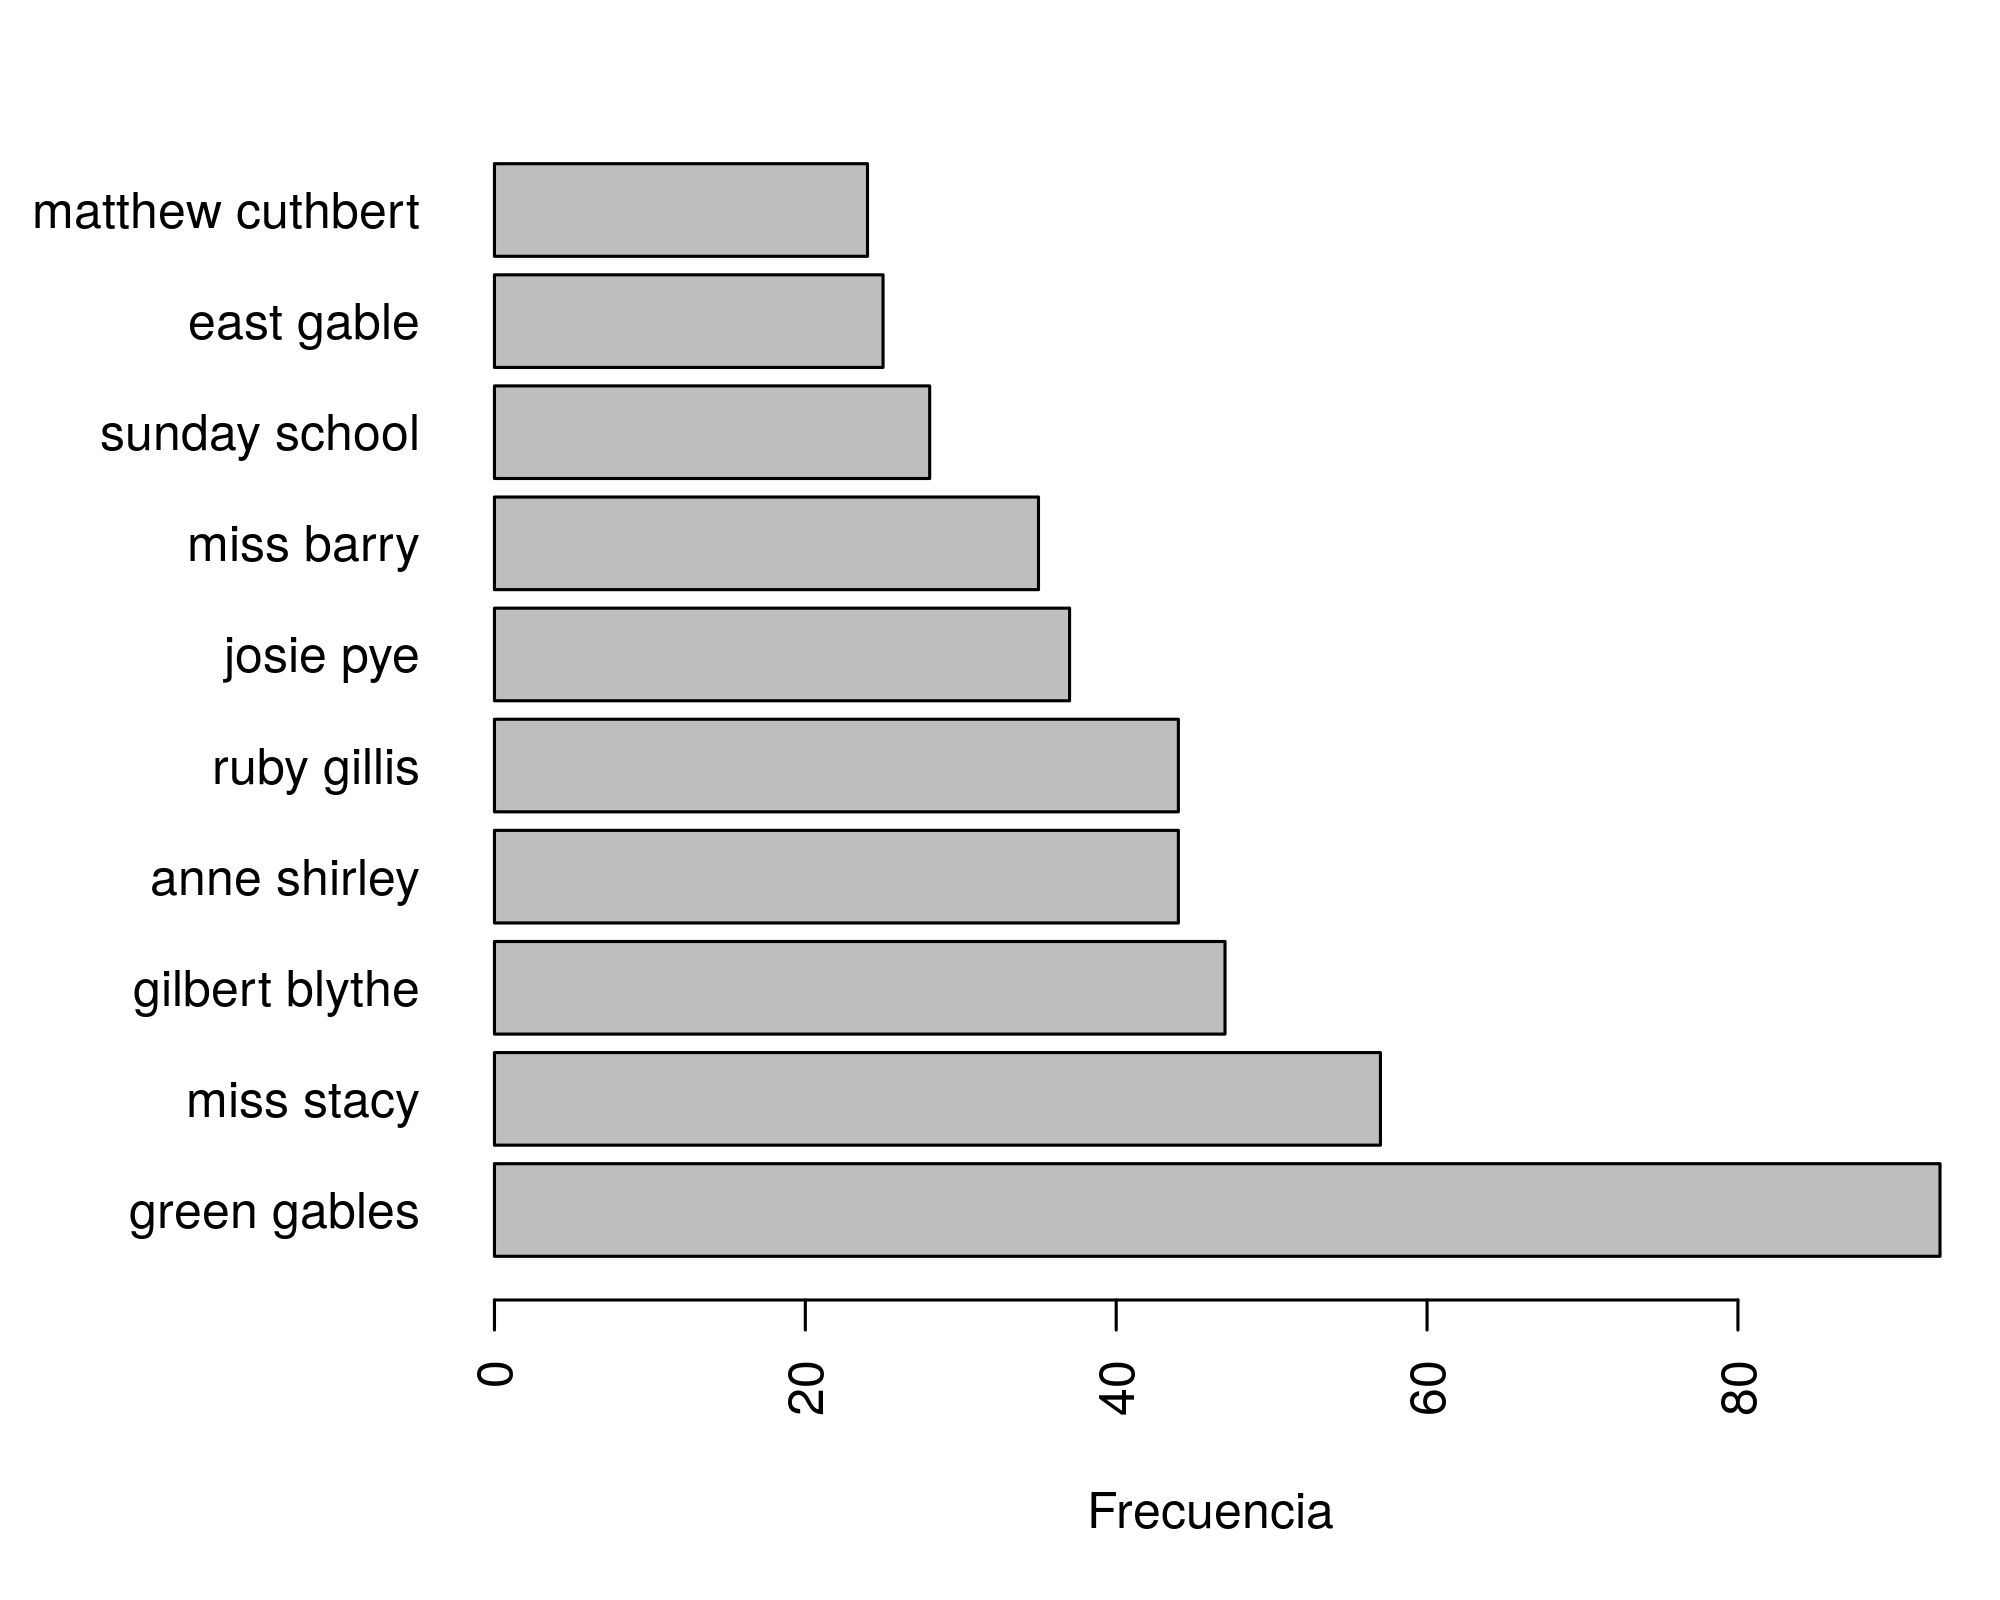
\includegraphics[scale=0.7]{bigrama.png}
		\caption{Bigramas con mayor frecuencia en el texto filtrado.}
		\label{bigrama_barplot}
	\end{figure}
	
\bibliographystyle{plain}
\bibliography{biblio}



\end{document}

